\documentclass[]{beamer}
\usetheme{Singapore}
\usepackage{physics}
\usepackage[absolute,overlay]{textpos}
\usepackage{graphicx}
\usepackage{tikzit}

\setbeamertemplate{footline}[frame number]

\input{computation.tikzdefs}
\input{computation.tikzstyles}

\title{A novel notation for quantum cryptography}
\subtitle{Applications to some recent quantum cryptographic protocols and their equivalences}
\author{Zef Wolffs \\ External Research Supervisor: Boris Škorić \\ Internal Thesis Advisor: Jacco de Vries }

\expandafter\def\expandafter\insertshorttitle\expandafter{%
	\insertshorttitle\hfill%
	\insertframenumber\,/\,\inserttotalframenumber}

\begin{document}

\maketitle

\begin{frame}
\frametitle{Outline}

\begin{itemize}

\item Introduction
	\begin{itemize}
		\item Quantum Information
		\item Quantum Cryptography
		\item The Diagrammatic Notation
		\item The Aim
	\end{itemize}

\item The Classical One Time Pad

\item The Quantum One Time Pad
	\begin{itemize}
		\item Quantum Teleportation and Quantum One Time Pad Equivalence
	\end{itemize}

\item Quantum Key Recycling

\item Discussion and Conclusions

\item Questions

\item References

\end{itemize}
\end{frame}

\section{Introduction}

\begin{frame}
	\centering 
	\Huge
	\usebeamercolor[fg]{frametitle}{Introduction}
\end{frame}

\subsection{Quantum Information}

\begin{frame}
	\frametitle{Quantum Information}
	\begin{columns}
		\begin{column}{0.5\textwidth}
		\begin{itemize}
			\item The classical bit vs. the qubit
			\vspace{2cm}
			\item Encoding and decoding
		\end{itemize}
		\end{column}
		\begin{column}{0.5\textwidth}  %%<--- here
			\begin{center}
				\begin{textblock*}{10cm}(3cm,3cm)
				
\includegraphics[width=0.05\textwidth]{ClassicalBit.png}
				\end{textblock*}
				\begin{textblock*}{5cm}(8cm,2.6cm)
				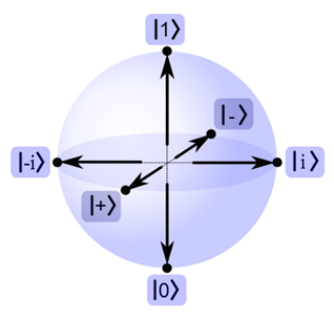
\includegraphics[width=0.5\textwidth]{QuantumBit.png}
				\end{textblock*}
				\begin{textblock*}{5cm}(7.1cm,5cm)
				\tiny	\textit{Representation of a classical bit (Left) and a qubit (right) \cite{Pomorski2018}.}
				\end{textblock*}
			%	\begin{textblock*}{7cm}(6.2cm,6cm)
			%		%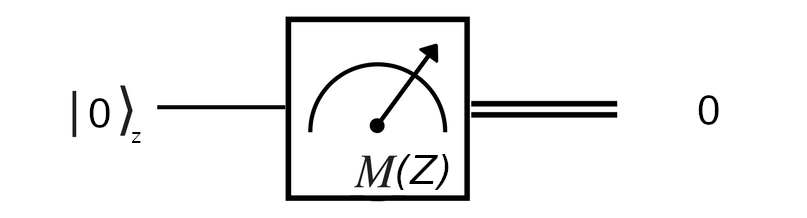
\includegraphics[width=0.5\textwidth]{MeasureInZ.png}
			%	\end{textblock*}
			%	\begin{textblock*}{7cm}(6.2cm,7cm)
			%	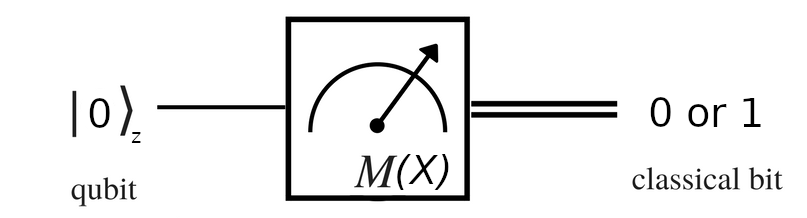
\includegraphics[width=0.5\textwidth]{MeasureInX.png}
			%	\end{textblock*}
			%	\begin{textblock*}{5cm}(7.2cm,8.1cm)
			%	\tiny	\textit{Measuring $\ket{0}_z$ in the Z and X bases \cite{Mishra2019}.}
			%	\end{textblock*}
			\end{center}
		\end{column}
	\end{columns}
\end{frame}

\subsection{Quantum Cryptography}

\begin{frame}
	\frametitle{Quantum Cryptography}
	\begin{columns}
		\begin{column}{0.6\textwidth}
				\begin{itemize}
				\item Quantum cryptographic protocols: Sending a message securely using quantum mechanics
				\vspace{2cm}
				\item Dirac notation is not very intuitive
				\end{itemize}
		\end{column}
	\begin{column}{0.5\textwidth}
		\begin{textblock*}{10cm}(7.4cm,2.8cm)
			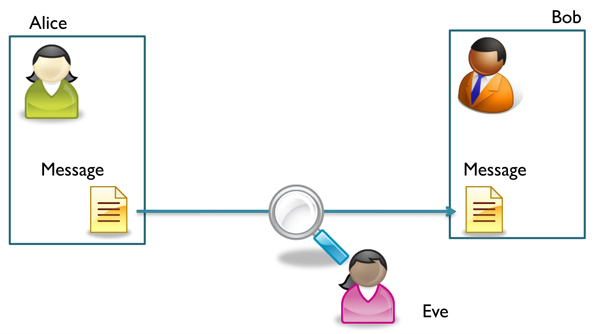
\includegraphics[width=0.5\textwidth]{AliceEveBob.png}
		\end{textblock*}
	\begin{textblock*}{6cm}(7.3cm,5.7cm)
		\tiny	\textit{Alice, Bob, and Eve's roles in (quantum) cryptographic protocols \cite{Cunche2011}.}
	\end{textblock*}
	\end{column}
	\end{columns}
\end{frame}

\subsection{The Diagrammatic Notation}

\begin{frame}
	\frametitle{The Diagrammatic Notation}
		\begin{textblock*}{12cm}(7cm,2.6cm)
		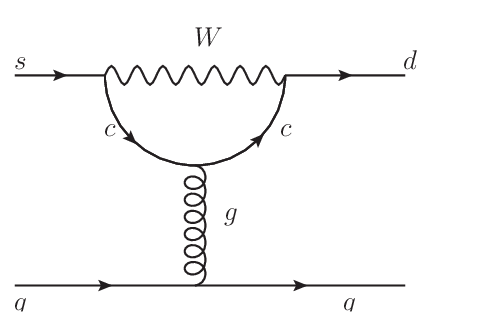
\includegraphics[width=0.5\textwidth]{PenguinDiagram.png}
	\end{textblock*}
	\begin{textblock*}{6cm}(1.6cm,6.9cm)
	\tiny	\textit{Diagrams in ecology: food webs \cite{Glaser}.}
	\end{textblock*}
	\begin{textblock*}{6cm}(7.2cm,6.9cm)
		\tiny	\textit{Diagrams in particle physics: Feynman diagrams \cite{Vos}.}
	\end{textblock*}
		\begin{textblock*}{12cm}(0.5cm,2.8cm)
		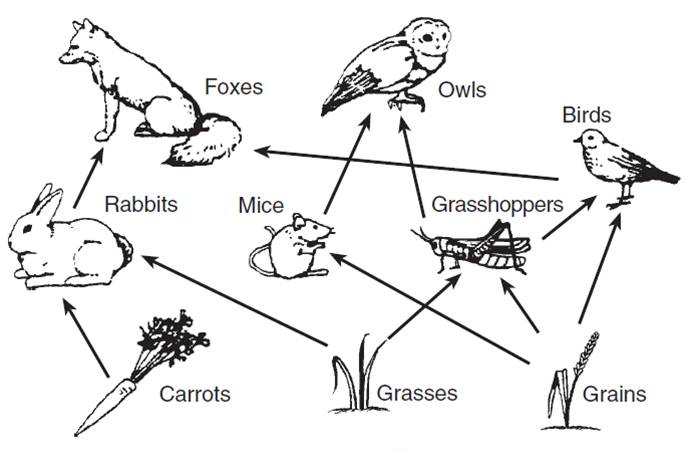
\includegraphics[width=0.5\textwidth]{FoodWeb.png}
	\end{textblock*}
\end{frame}

\begin{frame}
	\frametitle{The Dagrammatic Notation}
	\begin{columns}
		\begin{column}{0.5\textwidth}
			\begin{itemize}
			\item Proposed by Coecke and Kissinger in 2017, in \textit{Picturing Quantum Processes} \cite{Coecke2017}. 
			\end{itemize}
		\end{column}
		\begin{column}{0.5\textwidth}
			
		\end{column}
	\end{columns}
	 \begin{textblock*}{6cm}(8cm,3.9cm)
	 	\tikzfig{QAaSBProofSetupReal1X}
	 \end{textblock*}
\end{frame}

\subsection{Aim}

\begin{frame}
	\frametitle{The Aim}
	\begin{itemize}
		\item Taking into account the rising popularity of quantum cryptography and the fact that its current notation is insufficient for describing it intuitively we want to give the diagrammatic method a place in the field of quantum cryptography by...
		\vspace{0.6cm}
		\begin{enumerate}
			\item Writing a short handbook-style introduction to this notation for physicists reluctant to read the entire book \textit{Picturing Quantum Processes \cite{Coecke2017}.}
			\vspace{0.6cm}
			\item Constructing some recent quantum cryptographic developments and protocols in this new notation.
		\end{enumerate}
	\end{itemize}
\end{frame}

\section{The Classical One Time Pad}
\begin{frame}
	\centering 
	\Huge
	\usebeamercolor[fg]{frametitle}{The Classical One Time Pad}
\end{frame}
\begin{frame}
	\frametitle{The Classical One Time Pad}
	~~~~~~~~~~~~~Ideal situation:  ~~~~~~~~~~~~~~~~~ Real situation:
	\begin{equation}
	\tikzfig{BeamerOTP1} ~~~~~~~~~~~~~~~~~~~ \tikzfig{BeamerOTP2}
 	\end{equation}
\end{frame}

\begin{frame}
	\frametitle{The Classical One Time Pad}
	\begin{itemize}
	\item The One Time Pad solution: xor with secret random variable k
	\vspace{0.5cm}
	\end{itemize}
\begin{equation}
	\tikzfig{BeamerOTP3} = \tikzfig{BeamerOTP4} %= \tikzfig{BeamerOTP5}
\end{equation}
\end{frame}

\begin{frame}
	\frametitle{The Classical One Time Pad}
	\begin{itemize}
	\item If Eve does not interfere, communication should be
	provably correct.
	\end{itemize}
\begin{equation}
	\begin{split}
	\tikzfig{BeamerOTP6} = \tikzfig{BeamerOTP6A} = \tikzfig{BeamerOTP7} \\ = \tikzfig{BeamerOTP8} = \tikzfig{BeamerOTP9} \approx \tikzfig{BeamerOTP10}
	\end{split} 
\end{equation}
\end{frame}

\section{The Quantum One Time Pad}
\begin{frame}
	\centering 
	\Huge
	\usebeamercolor[fg]{frametitle}{The Quantum One Time Pad}
\end{frame}
\begin{frame}
	\frametitle{The Quantum One Time Pad}
	The Quantum One Time Pad ~~~~~~~ The Classical One Time Pad
	\begin{equation}
	\tikzfig{BeamerQOTP} ~~~~~~~~~~~~ \tikzfig{BeamerQOTPA}
	\end{equation}
\end{frame}

\begin{frame}
	\frametitle{The Quantum One Time Pad}
	The Quantum One Time Pad ~~~~~~~ The Classical One Time Pad
	\begin{equation}
	\tikzfig{BeamerQOTPDotted} ~~~~~~~~~~~~ \tikzfig{BeamerQOTPADotted}
	\end{equation}
\end{frame}

\subsection{Equivalence: Quantum Teleportation}

\begin{frame}
	\frametitle{Quantum Teleportation and Quantum One Time Pad Equivalence}
	~~~~~~~~~~~~~~~~~~~~~~~~~Quantum Teleportation
	\begin{equation}
	\tikzfig{QuantumTeleportation0}
	\end{equation}
\end{frame}

\begin{frame}
	\frametitle{Quantum Teleportation and Quantum One Time Pad Equivalence}
~~~~~~~~~	Quantum Teleportation ~~~~ The Quantum One Time Pad
	\begin{equation}
	\tikzfig{QuantumTeleportationNoLine1} ~~~~~~=~~~~~~ \tikzfig{BeamerQOTP1} %\tikzfig{BeamerQOTP2}
	\end{equation}
\end{frame}

\section{Quantum Key Recycling}
\begin{frame}
	\centering 
	\Huge
	\usebeamercolor[fg]{frametitle}{Quantum Key Recycling}
\end{frame}
\begin{frame}
	\frametitle{Quantum Key Recycling}
	\begin{equation}
	\tikzfig{QKRGeneralX}
	\end{equation}
\end{frame}

\begin{frame}
	\frametitle{Quantum Key Recycling}
	\begin{itemize}
		\item Security proof for quantum key recycling in the noiseless case, the starting point:
		\vspace{0.5cm}
	\end{itemize}
	\begin{equation}
		\tikzfig{BeamerQKR} = \tikzfig{BeamerQKR1} 
	\end{equation}
\end{frame}

\begin{frame}
	\frametitle{Quantum Key Recycling}
	\begin{itemize}
		\item With a lot of steps in between, the end result becomes:
		\vspace{0.5cm}
	\end{itemize}
	\begin{equation}
	\tikzfig{BeamerQKR2}
	\end{equation}
		\begin{itemize}
		\item In words: Eve's part of the diagram separates entirely from Alice and Bob's communication channel!
	\end{itemize}
\end{frame}
\section{Discussion and Conclusions}
\begin{frame}
	\centering 
	\Huge
	\usebeamercolor[fg]{frametitle}{Discussion and Conclusions}
\end{frame}
\begin{frame}
	\frametitle{Discussion and Conclusions}
	\begin{itemize}
		\item What novel things did we achieve in this thesis?\pause
		\begin{itemize}
			\item Wrote the first short \textbf{handbook-style introduction} to the diagrammatic notation\pause
			\item Developed the \textbf{classical One Time Pad} diagrammatically and showed that it both works and is secure\pause
			\item Developed the \textbf{quantum One Time Pad} diagrammatically and showed that it both works and is secure\pause
			\item Showed that \textbf{Quantum Teleportation} is equivalent to the quantum One Time Pad, and therefore also works and is secure\pause
			\item Developed \textbf{Quantum Key Recycling} diagrammatically, included a fully fledged security proof and worked out equivalences from a recent paper \cite{Leermakers2019}
		\end{itemize}
	\end{itemize}
\end{frame}

\begin{frame}
	\frametitle{Discussion and Conclusions}
	\begin{itemize}
		\item Did this achieve the aims?\pause
		\begin{enumerate}
			\item Writing a short handbook-style introduction to this notation for physicists hesitant to read the entire book \textit{Picturing Quantum Processes \cite{Coecke2017}.}\pause \newline
			\textcolor{orange}{\textbf{Maybe, up to the reader to decide.}}\pause
			\vspace{0.8cm}
			\item Constructing some recent quantum cryptographic developments and protocols in this new notation.\pause \newline
			\textcolor{green}{\textbf{Yes!}}
		\end{enumerate}
	\end{itemize}
\end{frame}

\begin{frame}
	\frametitle{Discussion and Conclusions}
	\begin{itemize}
	\item Role of diagrammatic notation?
	\item More technical: classical channels have a basis?
	\begin{equation}
	\tikzfig{explicitgraywire} ~~~~~~~~~~~~~~ \tikzfig{explicitwhitewire}
	\end{equation}
	\end{itemize}
\end{frame}

\begin{frame}
	\frametitle{Discussion and Conclusions}
	\begin{itemize}
		\item In future research it would be interesting to...
		\begin{itemize}
			\item Develop a full security proof for Quantum Key Recycling with noise
			\item Generally work out more protocols and equivalences in this notation
		\end{itemize}
	\end{itemize}
\end{frame}

\begin{frame}
		\centering 
		\Huge
		\usebeamercolor[fg]{frametitle}{Questions?}
\end{frame}
\begin{frame}[shrink=1]
	\frametitle{References}
\setbeamertemplate{bibliography item}[text]
	\bibliographystyle{plain}
	\bibliography{library}
\end{frame}

\end{document}